
%Part 22: The End
\section{Конец\label{sec:part22}}

\subsection{Все сделано}

%Whew! Thank you for sticking with me. When I started this series I didn’t realize it was going to be this long, or take this much time to make. But I have enjoyed creating it and hope you have enjoyed reading it.
На создание всех глав было потрачено много времени, но надеюсь, что 
вам понравилось.

%Now that I have finished, I will look into the possibility of generating a PDF format. No promises, though.


%I would like to conclude with a few suggestions on how to continue your Twisted education.
Далее несколько предложений по поводу дальнейшего изучения Twisted.

\subsection{Дальнейшее чтение}

%First, I would recommend reading the Twisted online documentation. Although it is much-maligned, I think it’s better than it is often given credit for.

Во-первых, рекомендуется почитать 
\href{http://twistedmatrix.com/trac/wiki/Documentation}{документацию на сайте}\footnote[1]{http://twistedmatrix.com/trac/wiki/Documentation}.


%If you want to use Twisted for web programming, then Jean-Paul Calderone has a well-regarded series called “Twisted Web in 60 Seconds“. I suspect it will take a little longer than that to read, though.
Если вы хотите использовать Twisted для web программирования, то 
есть хорошая книга Jean-Paul Calderone
\href{http://jcalderone.livejournal.com/50562.html}{<<Twisted Web in 60 Seconds>>}\footnote[2]{http://jcalderone.livejournal.com/50562.html}. Хотя, думается, что на прочтение вам 
потребуется немного больше времени. 


%There is also a Twisted Book, which I can’t say much about as I haven’t read it.
Также есть 
\href{http://www.amazon.com/gp/product/0596100329?ie=UTF8\&tag=jpcalsjou-20\&linkCode=as2\&camp=1789\&creative=9325\&creativeASIN=0596100329}{Twisted Book}\footnote[3]{http://www.amazon.com/gp/product/0596100329?ie=UTF8\&tag=jpcalsjou-20\&linkCode=as2\&camp=1789\&creative=9325\&creativeASIN=0596100329}.


%But more important than any of those, I think, is to read the Twisted source code. Since that code is written by people who know Twisted very well, it is an excellent source of examples for how do to things the “Twisted Way”.
Но важнее, чем все остальное, - это 
\href{http://twistedmatrix.com/trac/browser/trunk}{сами исходники Twisted}. Поскольку 
код написан людьми, которые очень хорошо знают Twisted, и это отличный 
источник примеров создания программ <<способом Twisted>>.


\subsection{Упражнения}

\begin{enumerate}

%   1. Port a synchronous program you wrote to Twisted.
\item Портируйте какую-нибудь вашу синхронную программу на Twisted.

%   2. Write a new Twisted program from scratch.
\item Напиши новую Twisted программу с нуля.

%   3. Pick a bug from the Twisted bug database and fix it. Submit a patch to the Twisted developers. Don’t forget to read about the process for making your contribution.
\item Выберите ошибку из \href{http://twistedmatrix.com/trac/report}{базы данных Twisted багов}\footnote[4]{http://twistedmatrix.com/trac/report} и исправьте его. 
Предоставьте patch разработчикам Twisted. Не забудьте 
прочитать про то, как можно 
\href{http://twistedmatrix.com/trac/wiki/ContributingToTwistedLabs}{посодействовать проекту}\footnote[5]{http://twistedmatrix.com/trac/wiki/ContributingToTwistedLabs}.

\end{enumerate}


%The End, Really
\subsection{Действительно конец}

%Happy Hacking!
Удачного программирования!

% fig47
\begin{figure}[h]
\begin{center}
    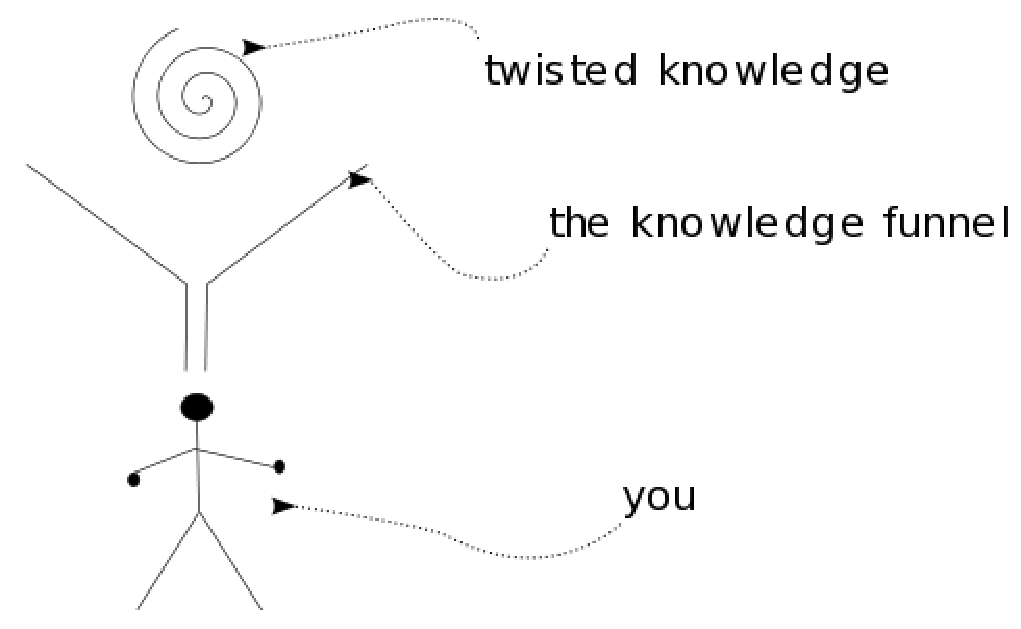
\includegraphics[width=1.\textwidth]{images/theend.pdf}
    \caption{Конец\label{fig:theend}}
\end{center}
\end{figure}


